\chapter{Installation der Meißner Anwendung}
\section{Voraussetzungen}
Dieses Installationsskript wurde für Debian entwickelt. Unter anderen Distributionen sind ähnliche Schritte notwendig, jedoch werden diese nicht von dem Shell Script übernommen.

\paragraph{Testsystem und Dauer der Installation}
Auf dem Testsystem war ein Kern einer Intel i5 2450M, 1 GB DDR3 Arbeitsspeicher und eine DSL 16000 Internetleitung verfügbar. Als Hostsystem wurde Linux Mint 15 verwendet, welches mit \emph{debootstrap} ein unverändertes Debian System installiert hatte. Über \emph{chroot} wurde dann ein Benutzer mit \emph{sudo}-Rechten eingerichtet, welcher das Shell Script schließlich aufgerufen hat.\par 

Für die Installation werden ca. 320 MB heruntergeladen. Darin enthalten sind allerdings alle notwendigen Pakete für einen Webserver und WebSocket Server sowie \emph{gcc, g++, make und configure}, um node\emph{node.js} aus den Quellen zu kompilieren.\par

Mit dieser Konfiguration wurden für die Installation 15 Minuten benötigt.

\section{Beschreibung}
Die Installation beginnt mit einem Update der Distribution auf die aktuellste Version. Danach wird ein LAMP-Server installiert und konfiguriert, gefolgt von der Installation der aktuellsten node.js Version. Letzteres muss vom Server kompiliert werden und nimmt daher einige Zeit in Anspruch.

\section{Installation von LAMP}
Zu Beginn der Installation ist es notwendig sich im gleichen Verzeichnis zu befinden, wie das Shell Script. Von dort aus führt man folgenden Befehl aus:

\begin{lstlisting}
	sudo sh install.sh
\end{lstlisting}

\subsection{MySQL}
Danach folgen einige Benutzereingaben, die auf den folgenden Screenshots zu sehen sind:
\begin{figure}[!ht]
	\centering
	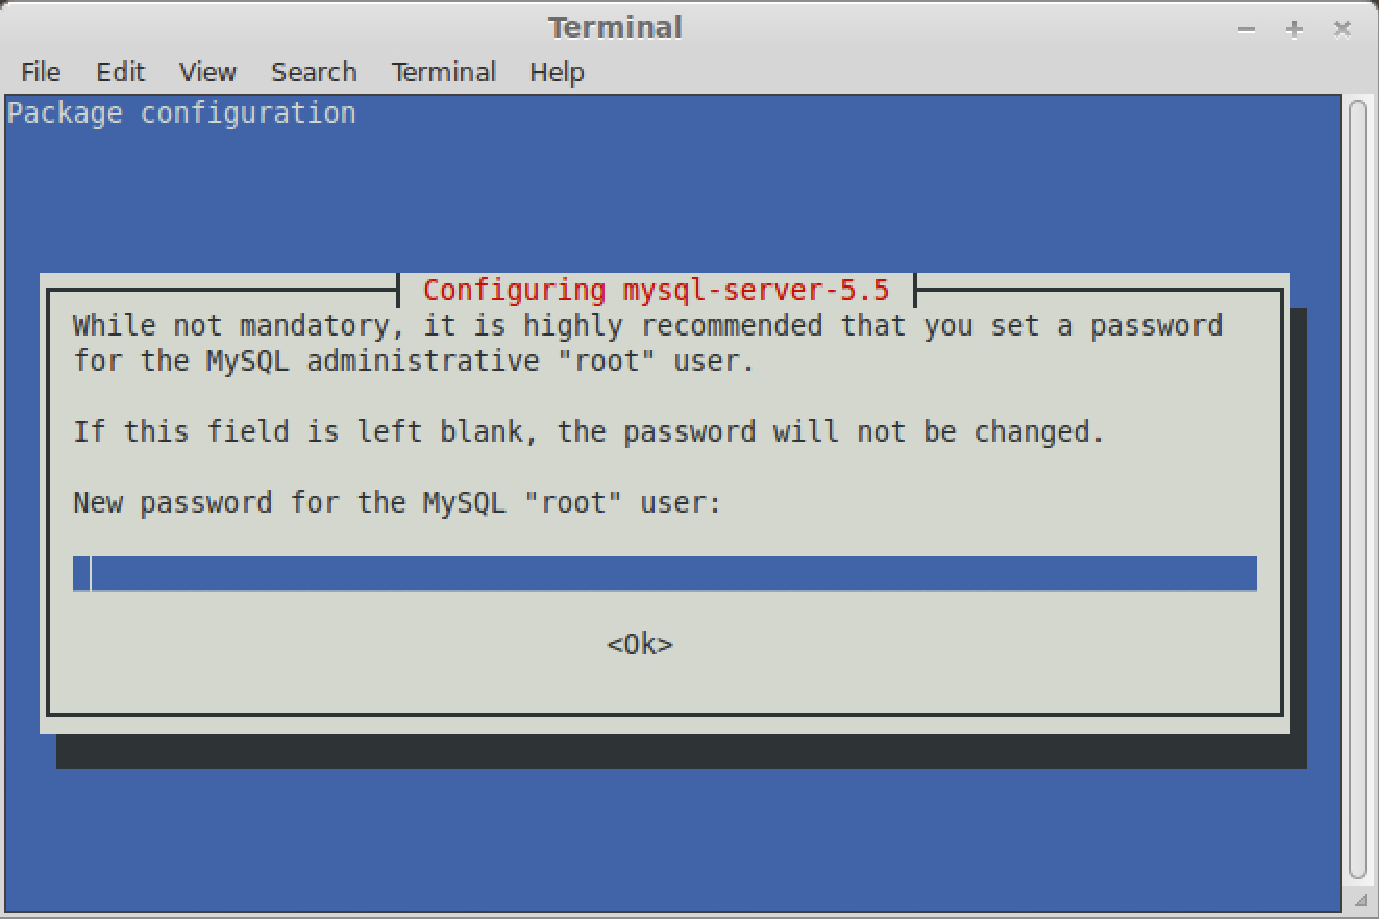
\includegraphics[width=15cm]{fig/configuring_mysql}
	\caption{Eingabe des root Passworts für die MySQL Datenbank}
\end{figure}
\par

Dieses Passwort muss nach der Eingabe noch einmal bestätigt werden.\par
\newpage
\subsection{phpmyadmin}
Bei der Installation von phpmyadmin erscheint folgender Dialog:
\begin{figure}[!ht]
	\centering
	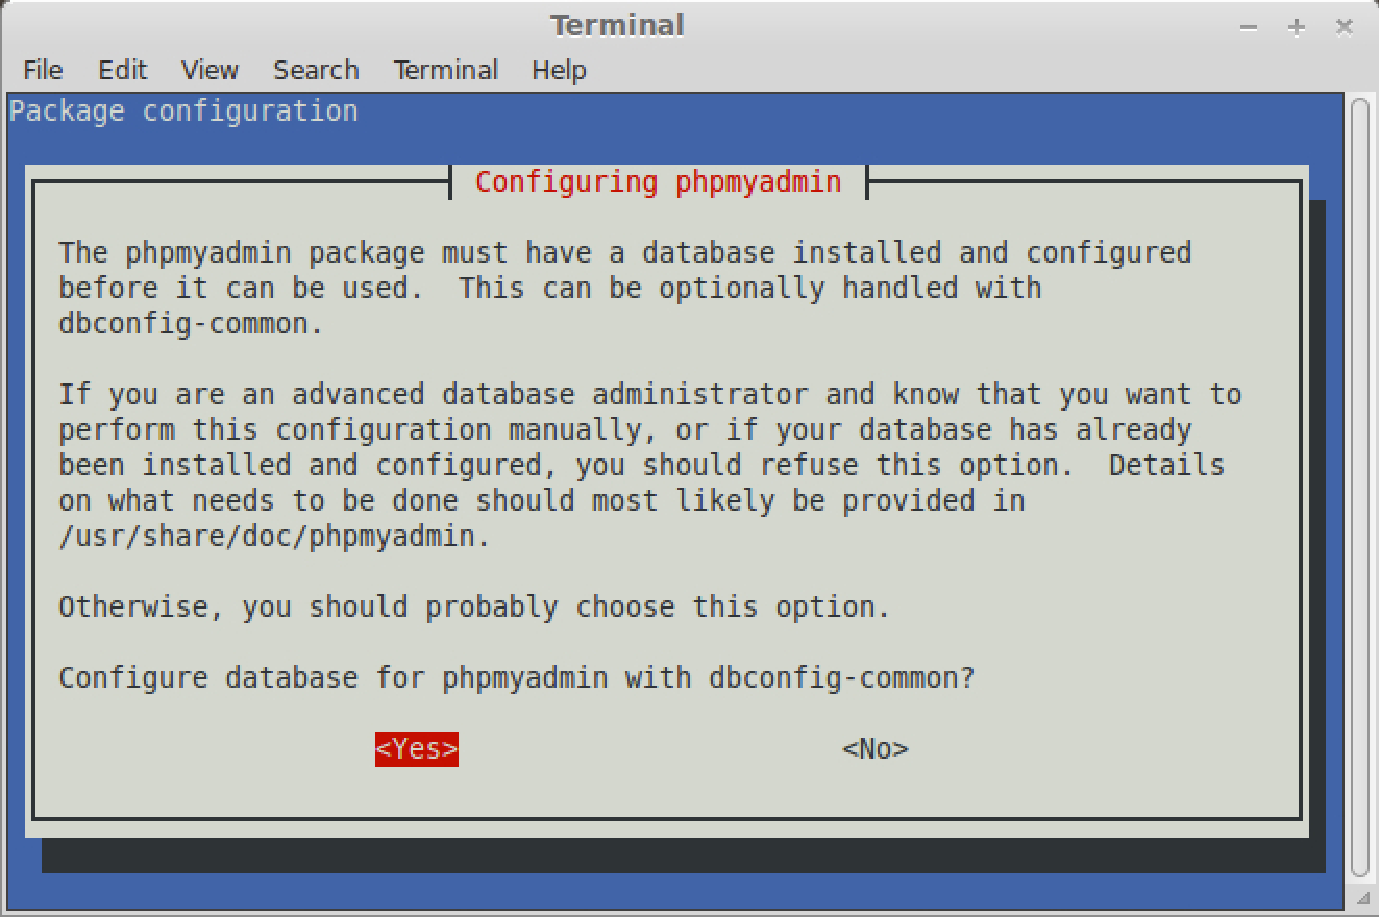
\includegraphics[width=15cm]{fig/configure_phpmyadmin}
	\caption{Eingabe des root Passworts für phpmyadmin}
\end{figure}

%%%%%%%%%%%%%%%%%%%%%%%%%%%%%%%%%%%

\newpage
\section{Installation von node.js}
Da es keine vorgefertigten Pakete von node.js gibt, muss das Skript sich die aktuellste Version von dem Server des Entwicklers herunterladen und anschließend selbst compilieren. Dafür werden Pakete wie \emph{make, configure, gcc, g++} benötigt, die schon im ersten Schritt dieser Installation installiert wurden. 

%%%%%%%%%%%%%%%%%%%%%%%%%%%%%%%%%%%
%%%%%%%%%%%%%%%%%%%%%%%%%%%%%%%%%%%%%%%%%%%%%%%%%%%%%%%%%%%%%%%%%%%%%%
%%%%%%%%%%%%%%%%%%%%%%%%%%%%%%%%%%%

\chapter{Eigene Anpassungen}
\section{Erzeugung eines neuen Models}
Um einen eigenen Bereich zu erzeugen, der später in der App verfügbar sein soll, können eigene Model, View und Controller entwickelt werden. Diese können im Ordner

\begin{itemize}
	\item[] \emph{meissner/app/\{Model, View, Controller\}}
\end{itemize}

angelegt werden.\par

Damit der View nun in das Layout eingebunden wird, muss der entsprechende Eintrag noch in der Navigation verlinkt werden:

\begin{itemize}
	\item[] \emph{meissner/app/View/Layouts/\{nav.ctp, mobilenav.ctp\}}
\end{itemize}

\section{Bearbeitung des Layouts}
Das Layout der Anwendung kann unter 

\begin{itemize}
	\item[] \emph{meissner/app/View/Layouts/\{default.ctp, mobile.ctp\}}
\end{itemize}

verändert werden. Dort befindet sich das Grundgerüst der Webanwendung. Stylesheets, JavaScripte, Navigation und so weiter können hier für alle Views eingebunden werden. 

\subsection{Bedeutung von webroot/}
In dem Ordner webroot werden Grafiken, Skripte, Stylesheets und andere Dateien gespeichert, die der Anwendung zur Verfügung gestellt werden sollen. 

\begin{itemize}
	\item[] \emph{meissner/app/webroot}
\end{itemize}

Von diesem Ort geht die Anwendung aus, wenn etwas eingebunden werden soll, das bedeutet wenn man im Layout die Datei \emph{css/stylesheet.css} aufrufen möchte, darf diese nicht in \emph{meissner/app/View/Layouts/css/stylesheet.css} liegen, sondern eben in \emph{meissner/app/webroot/css/stylesheet.css}. Das gilt auch für alle Bilder, Skripte und so weiter.\\
Das hat den Vorteil, dass alle Dateien zentral in einem Ordner gespeichert sind und nicht verteilt im cakePHP Framework zu suchen sind.

\subsection{Designs mit CSS}
Stylesheets können entsprechend im webroot-Verzeichnis gefunden werden:

\begin{itemize}
	\item[] \emph{meissner/app/webroot/css}
\end{itemize}

Standardmäßig laden die Desktop- und Mobilversion der Anwendung zuerst die \emph{main.css}, worin die gemeinsamen Styles definiert sind. Danach werden layoutspezifische Stylesheets nachgeladen, welche ebenfalls in diesem Ordner zu finden sind. 

\subsection{Einbindung von JavaScript}
Wie schon beschrieben, werden Skripte auch in \emph{webroot/js} gespeichert. Dann können Sie im Layout oder in den Views der App einfach mit folgendem Befehl geladen werden:

\begin{lstlisting}
  <script type="text/javascript" scr="js/javascript.js">
  </script>
\end{lstlisting}

Unabhängig des Pfades, in dem sich der View oder das Layout befindet, wird mit diesem Befehl immer im webroot-Verzeichnis nach der angegebenen Datei gesucht. Das erleichtert das Entwickeln neuer Views, da der Entwickler nicht mehr nachdenken muss, in welchem Ordner er sich gerade befindet.






